\documentclass[leqno]{article}
% Shared QBT/Soln pack preamble for resources.danieljsmith.org.
\usepackage{graphicx}
\usepackage{dsfont}
\usepackage{mathtools}
\usepackage{amssymb}
\usepackage{amsmath}
\usepackage{mleftright}
\usepackage{amsthm}
\usepackage{float}
\usepackage{ragged2e}
\usepackage{tensor}
\usepackage{fancyhdr}
\usepackage{empheq}
\usepackage[most]{tcolorbox}
\usepackage{enumitem}
\usepackage{dirtytalk}
\usepackage{marginnote}
\usepackage{microtype}
\usepackage[
  a4paper,
  left=0.8in,
  right=1in,
  top=1in,
  bottom=0.5in,
  headheight=14pt,
  headsep=0.4in
]{geometry}
\setlength{\parindent}{0cm}

% TikZ / PGFPlots
\usepackage{pgfplots}
\pgfplotsset{compat=1.18}
\usepgfplotslibrary{fillbetween, polar}
\usetikzlibrary{calc, positioning}
\usetikzlibrary{angles, quotes}
\usetikzlibrary{arrows.meta}
\usetikzlibrary{decorations.pathreplacing, decorations.markings}
\usetikzlibrary{patterns}
\usetikzlibrary{intersections}

% Links and contents. The contents follow the TMUA papers: compact entries,
% no dot leaders, and each question's mark total in grey after its label.
\usepackage{tocloft}
\tocloftpagestyle{fancy}
\setlength{\cftbeforesubsecskip}{2pt}
\setlength{\cftsubsecindent}{1.5em}
\setlength{\cftsubsecnumwidth}{0pt}
\renewcommand{\cftsubsecfont}{\small\color{black}}
\renewcommand{\cftsubsecpagefont}{\small\color{black}}
\renewcommand{\cftsubsecleader}{\hfill}
\usepackage[colorlinks=true,linkcolor=black,citecolor=magenta,urlcolor=black]{hyperref}%
\urlstyle{same}

% Pack macros
% \marks also adds its value to the current question's total in the .aux
% file, so the contents show each total from the second pass. The write
% happens at shipout, so a box typeset more than once counts once. The
% pack's mark total for the contents-page title is summed the same way.
\makeatletter
\newcount\djs@totalmarks
\newcommand{\djsAddMarks}[2]{%
  \global\advance\djs@totalmarks#2\relax
  \@ifundefined{djs@marks@#1}%
    {\expandafter\xdef\csname djs@marks@#1\endcsname{#2}}%
    {\expandafter\xdef\csname djs@marks@#1\endcsname
      {\the\numexpr\csname djs@marks@#1\endcsname+#2\relax}}}
\RenewDocumentCommand{\marks}{o m}{%
  \protected@write\@auxout{}{\string\djsAddMarks{\number\value{enumi}}{#2}}%
  \IfValueTF{#1}%
    {\marginnote{\raggedright\textbf{[#2]}}[#1]}%
    {\marginnote{\raggedright\textbf{[#2]}}}%
}
\makeatother

\newcommand{\vspacerule}[2]{%
  \par\vspace*{#1}%
  \noindent\hrulefill\par
  \vspace*{#2}%
}

\definecolor{scarlet}{RGB}{205, 40, 75}
% Site colours for the contents-page title: the accent, the rule colour, a
% stronger rule colour for the path separator, and the muted text colour.
\definecolor{djsBurgundy}{RGB}{118, 59, 67}
\definecolor{djsHairline}{RGB}{216, 213, 205}
\definecolor{djsSlash}{RGB}{170, 166, 158}
\definecolor{djsMuted}{RGB}{96, 101, 106}

% Worked-solution box, adapted from the TMUA worked-solutions box. A white breakable box with a left scarlet rule and no surrounding
% frame or tint. A part that breaks fills the rest of its page, so the rule
% runs to the bottom margin; the unbroken or last part ends in a short
% horizontal foot rule so a solution visibly stops. Unlike the TMUA box there
% is no answer label. The box does not grow to the left, so the rule sits at
% the text edge; growing to the right keeps the usable line width close to the
% old tcolorbox Solution box.
% Spacing inside the box: paragraphs are 6pt apart, so source blank lines show
% (solutions put one after each display and none between a lead-in and its
% display). Every display gets 6pt above and 10pt below, whatever the length
% of its lead-in line; align rows are spread by an 8pt \jot; solution parts
% are 14pt apart and sub-parts 8pt; \left and \right space like ordinary
% brackets (mleftright); no single line is stranded at a page break; and
% neither the Solution label nor the line before a list ends a page. No
% skip can shrink, so full pages are not squeezed.
\newtcolorbox{djsSolution}{%
  enhanced, breakable, frame hidden, sharp corners, colback=white,
  height fixed for=first and middle, height fill,
  extras unbroken and last={natural height},
  borderline west={2.2pt}{0pt}{scarlet},
  left=11pt, right=0pt, top=5pt, bottom=13pt,
  before skip=13pt, after skip=4pt,
  grow to right by=10mm,
  overlay unbroken and last={%
    \fill[scarlet] (frame.south west)
      rectangle ([xshift=3.5cm, yshift=2.2pt]frame.south west);},
  before upper={{\color{scarlet}\bfseries Solution}\par\nobreak\vspace{4pt}%
    \setlength{\parskip}{6pt plus 2pt}%
    \setlength{\abovedisplayskip}{6pt plus 2pt}%
    \setlength{\abovedisplayshortskip}{6pt plus 2pt}%
    \setlength{\belowdisplayskip}{10pt plus 2pt}%
    \setlength{\belowdisplayshortskip}{10pt plus 2pt}%
    \setlength{\jot}{8pt}%
    \setlist{parsep=6pt plus 2pt, topsep=6pt plus 2pt, beginpenalty=10000}%
    \setlist[enumerate,1]{itemsep=14pt plus 2pt}%
    \setlist[enumerate,2]{itemsep=8pt plus 2pt}%
    \mleftright
    \clubpenalty=10000 \widowpenalty=10000 \displaywidowpenalty=10000\relax}}

% Optional smaller figure inside a solution box. \scalebox shrinks node text
% with the drawing. Not applied to existing figures.
\newcommand{\SolnFigureScale}{0.85}
\newsavebox{\djsSolnFigureBox}
\newenvironment{djsSolutionFigure}
  {\par\vspace{4pt}\begin{center}\begin{lrbox}{\djsSolnFigureBox}}
  {\end{lrbox}\scalebox{\SolnFigureScale}{\usebox{\djsSolnFigureBox}}%
   \end{center}\vspace{2pt}\par}

\newcommand{\cxl}[2]{%
  \tikz[baseline=(X.base)]{%
    \node[inner sep=0pt, outer sep=0pt, text=#1] (X) {$#2$};
    \draw[#1, line width=0.4pt] (X.south west)--(X.north east);
  }%
}

% Page-style hook run at the contents page and each question's opening page.
% A no-op for QBT packs; \djsSolnHeader points it at the fancy header.
\newcommand{\djsQuestionPageStyle}{}

% A contents entry: "Question N" in a box wide enough for two digits, so the
% mark totals line up, then the total in grey. Bookmarks keep "Question N".
\makeatletter
\newlength{\djsTocLabelWidth}
\newcommand{\djsTocMarks}[1]{%
  \@ifundefined{djs@marks@#1}{}{%
    {\footnotesize\itshape\color{black!45}%
     \csname djs@marks@#1\endcsname~mark%
     \ifnum\csname djs@marks@#1\endcsname=1 \else s\fi}}}
\newcommand{\djsTocEntry}[1]{%
  \texorpdfstring
    {\settowidth{\djsTocLabelWidth}{Question 00}%
     \makebox[\dimexpr\djsTocLabelWidth+0.9em\relax][l]{Question #1}%
     \djsTocMarks{#1}}%
    {Question #1}}
\makeatother

% The question count for the contents-page title is written to the .aux at
% the end of the document, so it also appears from the second pass.
\newcounter{djsQuestions}
\newcommand{\questionitem}{%
  \djsQuestionPageStyle
  \item\phantomsection
  \stepcounter{djsQuestions}%
  \addcontentsline{toc}{subsection}{\protect\djsTocEntry{\number\value{enumi}}}%
}
\makeatletter
\newcommand{\djsSetQuestionCount}[1]{\gdef\djs@questioncount{#1}}
\AtEndDocument{\immediate\write\@auxout
  {\string\djsSetQuestionCount{\number\value{djsQuestions}}}}
\makeatother

\renewcommand{\contentsname}{Questions}

% \djsPackHeader[<link content tag>]{<left header>}; the tag says which
% document a click on the header link came from.
\newcommand{\djsPackHeader}[2][questions]{%
  \pagestyle{fancy}%
  \fancyhead{}%
  \fancyfoot{}%
  \renewcommand{\headrulewidth}{0.9pt}%
  \lhead{#2}%
  \chead{}%
  \rhead{\href{https://danieljsmith.org/?utm_source=pdf&utm_campaign=further-maths&utm_content=#1}{danieljsmith.org}}%
}

% The header's topic is also the contents-page title, under which a label
% says which booklet this is.
\newcommand{\djsPackTitle}{}
\newcommand{\djsBookletLabel}{}
\newcommand{\djsQbtHeader}[1]{%
  \djsPackHeader{#1}%
  \renewcommand{\djsPackTitle}{#1}%
  \renewcommand{\djsBookletLabel}{Questions by topic}%
}

% The colophon at the foot of page one, independent of the page style: the
% contents-page title's hairline led by a short scarlet rule, then the date on
% the left and a link to the site on the right, all inside the bottom margin.
% Its sizes are fixed, so it matches the TMUA papers' colophon. The document
% supplies the date; recompiling never changes it.
\makeatletter
\newcommand{\djsLastUpdated}[1]{%
  \AtBeginDocument{\AddToHookNext{shipout/foreground}{\djs@colophon{#1}}}}
\newcommand{\djs@colophon}[1]{%
  \put(0.8in,-\dimexpr\paperheight-0.47in\relax){%
    \makebox[0pt][l]{\color{djsHairline}%
      \rule[0.9pt]{\dimexpr\paperwidth-1.8in\relax}{0.6pt}}%
    \makebox[0pt][l]{\color{scarlet}\rule{3.5cm}{2.2pt}}}%
  \put(0.8in,-\dimexpr\paperheight-0.32in\relax){\makebox[0pt][l]{%
    \fontsize{9}{11}\selectfont Last updated #1}}%
  \put(\dimexpr\paperwidth-1in\relax,-\dimexpr\paperheight-0.32in\relax){%
    \makebox[0pt][r]{\fontsize{7}{8.5}\selectfont\color{djsMuted}%
      Latest version at \href{https://resources.danieljsmith.org/}%
        {\color{black}resources.danieljsmith.org}}}}
\makeatother

% Solutions packs show the header only on the contents page and each
% question's opening page, so it never appears part-way through a solution.
% \thispagestyle marks the next page shipped out, which is the question's
% page because every solution question starts after a \newpage.
\newcommand{\djsSolnHeader}[1]{%
  \djsPackHeader[solutions]{\textit{Solutions} - #1}%
  \pagestyle{empty}%
  \renewcommand{\djsQuestionPageStyle}{\thispagestyle{fancy}}%
  \renewcommand{\djsPackTitle}{#1}%
  \renewcommand{\djsBookletLabel}{Worked solutions}%
}

% \djsSitePath{<strand>}{<topic>}, called once after the header, names where
% the pack sits on the site; the contents-page title prints it above the pack
% title, e.g. CORE PURE / FURTHER CALCULUS. Without it the line is left out.
\makeatletter
\newif\ifdjs@sitepath
\newcommand{\djs@strand}{}
\newcommand{\djs@section}{}
\newcommand{\djsSitePath}[2]{%
  \djs@sitepathtrue
  \renewcommand{\djs@strand}{#1}%
  \renewcommand{\djs@section}{#2}%
}
\makeatother

% Further Mechanics packs call \djsMechanicsPack in their preamble, so that
% \djsFrontMatter prints the default value of g above the contents. The box
% keeps its own space above it (before skip is the whole gap below the title,
% not an addition to it). Without the box, \djsGravityNote is just extra space
% before the contents heading, bringing the gap above it close to the gap
% between the box and the heading on Further Mechanics pages.
\newcommand{\djsGravityNote}{\vspace{14pt}}
\newcommand{\djsMechanicsPack}{%
  \renewcommand{\djsGravityNote}{%
    \begin{tcolorbox}[sharp corners, colback=white, colframe=black,
      boxrule=1pt, left=8pt, right=8pt, top=6pt, bottom=6pt,
      before skip=20pt]
    {\bfseries Instructions}\par\vspace{4pt}
    Unless a question states otherwise, take $g = 9.8\,\mathrm{m\,s^{-2}}$
    wherever a numerical value of $g$ is required. Solutions also give final
    answers for $g = 10\,\mathrm{m\,s^{-2}}$ where these differ.
    \end{tcolorbox}%
    \vspace{16pt}}%
}

% Contents-page title: the site path in spaced burgundy capitals, the pack
% title, a hairline led by a short scarlet rule (the solution box's foot rule),
% then the booklet label with the question and mark counts. The counts come
% from the .aux, so they appear from the second pass.
\makeatletter
\newsavebox{\djs@eyebrowbox}
\newcommand{\djs@caps}[1]{\textls[180]{\MakeUppercase{#1}}}
\newcommand{\djs@eyebrow}{%
  \color{djsBurgundy}\footnotesize\bfseries
  \djs@caps{\djs@strand}%
  {\color{djsSlash}\hspace{0.55em}/\hspace{0.55em}}%
  \djs@caps{\djs@section}}
\newcommand{\djs@dot}{\hspace{0.45em}\textperiodcentered\hspace{0.45em}}
\newcommand{\djs@counts}{%
  \@ifundefined{djs@questioncount}{}{%
    \djs@questioncount~question\ifnum\djs@questioncount=1 \else s\fi
    \ifnum\djs@totalmarks>0
      \djs@dot\the\djs@totalmarks~mark\ifnum\djs@totalmarks=1 \else s\fi
    \fi}}
\newcommand{\djsContentsTitle}{%
  \ifdjs@sitepath
    \sbox\djs@eyebrowbox{\djs@eyebrow}%
    \ifdim\wd\djs@eyebrowbox>\linewidth
      \@latex@warning@no@line{The \string\djsSitePath\space line is wider
        than the text, so it wraps. Shorten its topic}%
    \fi
    {\raggedright\djs@eyebrow\par}%
    \vspace{7pt}%
  \fi
  {\raggedright\fontsize{24.88}{28}\selectfont\djsPackTitle\par}%
  \vspace{9pt}%
  \noindent\makebox[0pt][l]{\color{djsHairline}\rule[0.9pt]{\linewidth}{0.6pt}}%
  {\color{scarlet}\rule{3.5cm}{2.2pt}}\par
  \vspace{5pt}%
  {\small\color{djsMuted}\djsBookletLabel\hfill\djs@counts\par}%
  \vspace{8pt}%
}
\makeatother

\newcommand{\djsFrontMatter}{%
  \djsQuestionPageStyle
  \vspace*{6pt}%
  \djsContentsTitle
  \djsGravityNote
  \tableofcontents
  \newpage
}


\djsQbtHeader{Oblique Collisions of Smooth Spheres}
\djsSitePath{Further Mechanics}{Momentum \& Collisions}
\djsMechanicsPack
\djsLastUpdated{13 October 2026}

\begin{document}
\djsFrontMatter
\begin{enumerate}[
  label=\textbf{\arabic*.},
  leftmargin=*,
  topsep=0pt,
  partopsep=0pt,
  parsep=0pt
]

% ---- Question 1 ----
\questionitem
% [Source: _QBT__Oblique_Collisions_of_Smooth_Spheres, Q1]

\begin{figure}[H]
    \centering
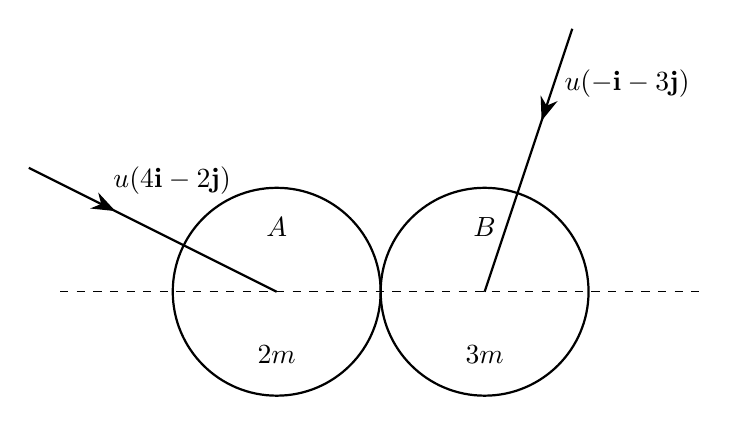
\begin{tikzpicture}[scale=1.1]
\def\rad{1.2}
\def\raylen{3.2}
\def\axisextra{1.3}
\pgfmathsetmacro{\angA}{180-atan(1/2)}
\pgfmathsetmacro{\angB}{atan(3)}
\coordinate (A) at (0,0);
\coordinate (B) at ($(A)+(2*\rad,0)$);
\coordinate (Left) at ($(A)+({-\rad-\axisextra},0)$);
\coordinate (Right) at ($(B)+({\rad+\axisextra},0)$);
\coordinate (StartA) at ($(A)+(\angA:\raylen)$);
\coordinate (StartB) at ($(B)+(\angB:\raylen)$);
\draw[dashed,black] (Left) -- (Right);
\foreach \p/\mass in {A/2m,B/3m} {
  \draw[thick,black] (\p) circle (\rad);
  \node at ($(\p)+(0,0.62*\rad)$) {$\p$};
  \node at ($(\p)+(0,-0.60*\rad)$) {$\mass$};
}
\draw[thick,black,postaction={decorate},decoration={markings,mark=at position 0.35 with {\arrow{Stealth[length=3mm]}}}] (StartA) -- (A) node[pos=0.30,above right] {$u(4\mathbf{i}-2\mathbf{j})$};
\draw[thick,black,postaction={decorate},decoration={markings,mark=at position 0.35 with {\arrow{Stealth[length=3mm]}}}] (StartB) -- (B) node[pos=0.30,above right,xshift=3pt] {$u(-\mathbf{i}-3\mathbf{j})$};
\end{tikzpicture}
\end{figure}


Two uniform smooth spheres $A$ and $B$, of equal radius and masses $2m$ and $3m$ respectively, collide on a smooth horizontal surface. The unit vector $\mathbf{i}$ points along the line of centres from $A$ towards $B$ at impact, and $\mathbf{j}$ is perpendicular to $\mathbf{i}$ in the plane of the surface, as indicated by the velocity directions in the diagram above. \\

Immediately before the collision, their velocities are
\[
\mathbf{u}_A=u(4\mathbf{i}-2\mathbf{j}),\qquad \mathbf{u}_B=u(-\mathbf{i}-3\mathbf{j})
\] \\
where $u>0$. Immediately after the collision, the direction of motion of $A$ is perpendicular to its direction of motion immediately before the collision. \\
\begin{enumerate}[label=\textbf{(\alph*)}]
\item Find the velocity of $A$ immediately after the collision, in terms of $u$. \marks{3} \\
\item Find the coefficient of restitution between the spheres and the percentage loss in their total kinetic energy. Give the percentage to three significant figures. \marks{4} \\
\end{enumerate}

\newpage

% ---- Question 2 ----
\questionitem
% [Source: _QBT__Oblique_Collisions_of_Smooth_Spheres, Q2]

\begin{figure}[H]
    \centering
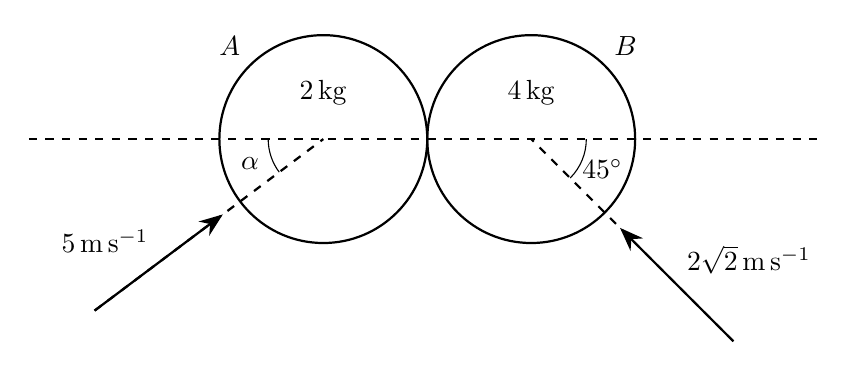
\begin{tikzpicture}[scale=1.1]
\def\rad{1.2}
\def\raylen{3.3}
\def\arrowstop{1.45}
\def\extension{3.4}
\pgfmathsetmacro{\alphaang}{atan(3/4)}
\pgfmathsetmacro{\adir}{180+\alphaang}
\def\bdir{315}
\coordinate (A) at (0,0);
\coordinate (B) at ($(A)+(2*\rad,0)$);
\coordinate (Left) at ($(A)+(-\extension,0)$);
\coordinate (Right) at ($(B)+(\extension,0)$);
\coordinate (Aleft) at ($(A)+(180:\rad)$);
\coordinate (Bright) at ($(B)+(0:\rad)$);
\coordinate (Astart) at ($(A)+(\adir:\raylen)$);
\coordinate (Aend) at ($(A)+(\adir:\arrowstop)$);
\coordinate (Bstart) at ($(B)+(\bdir:\raylen)$);
\coordinate (Bend) at ($(B)+(\bdir:\arrowstop)$);
\draw[thick, black, dashed] (Left) -- (Right);
\draw[thick, black] (A) circle (\rad);
\draw[thick, black] (B) circle (\rad);
\foreach \s in {A,B} {
  \draw[thick, black, dashed] (\s start) -- (\s);
}
\draw[-{Stealth[length=3mm]}, thick, black] (Astart) -- (Aend) node[midway, above left] {$5\,\mathrm{m\,s^{-1}}$};
\draw[-{Stealth[length=3mm]}, thick, black] (Bstart) -- (Bend) node[midway, above right] {$2\sqrt{2}\,\mathrm{m\,s^{-1}}$};
\pic["$\alpha$", draw, angle radius=7mm, angle eccentricity=1.4] {angle=Aleft--A--Astart};
\pic["$45^\circ$", draw, angle radius=7mm, angle eccentricity=1.4] {angle=Bstart--B--Bright};
\node[above left] at ($(A)+(135:\rad)$) {$A$};
\node[above right] at ($(B)+(45:\rad)$) {$B$};
\node at ($(A)+(0,0.45*\rad)$) {$2\,\mathrm{kg}$};
\node at ($(B)+(0,0.45*\rad)$) {$4\,\mathrm{kg}$};
\end{tikzpicture}
\end{figure}


Two smooth uniform spheres $A$ and $B$, of equal radius and masses $2\,\mathrm{kg}$ and $4\,\mathrm{kg}$ respectively, collide on a smooth horizontal surface. The diagram above shows a plan view at the instant of contact. \\

Immediately before the collision, sphere $A$ has speed $5\,\mathrm{m\,s^{-1}}$ and its velocity makes an acute angle $\alpha$ with the line of centres, where $\tan\alpha=\dfrac{3}{4}$. Sphere $B$ has speed $2\sqrt{2}\,\mathrm{m\,s^{-1}}$ and its velocity makes an angle of $45^\circ$ with the line of centres. Their velocity components along the line of centres are directed towards each other, and their perpendicular components are directed towards the same side of this line, as shown in the diagram above. \\

Immediately after the collision, the velocities of the two spheres are perpendicular. \\

Determine the coefficient of restitution between the spheres and the magnitude of the impulse exerted on $A$ during the collision. Give both answers in exact form. \marks{8} \\

\newpage

% ---- Question 3 ----
\questionitem
% [Source: _QBT__Oblique_Collisions_of_Smooth_Spheres, Q3]

\begin{figure}[H]
    \centering
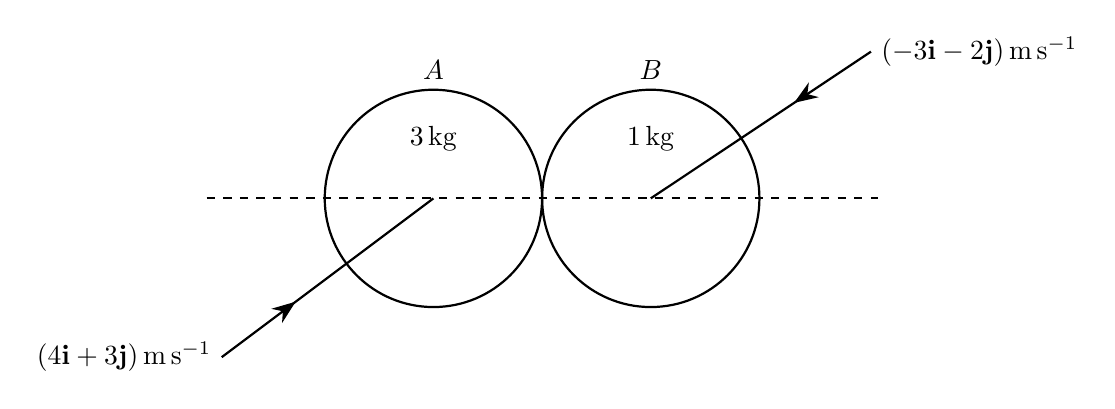
\begin{tikzpicture}[scale=1.2]
\def\rad{1.15}
\def\incomingLen{2.8}
\def\axisExtension{2.4}
\pgfmathsetmacro{\aRayAngle}{180+atan2(3,4)}
\pgfmathsetmacro{\bRayAngle}{atan2(2,3)}
\coordinate (A) at (0,0);
\coordinate (B) at ($(A)+(2*\rad,0)$);
\coordinate (Left) at ($(A)+(-\axisExtension,0)$);
\coordinate (Right) at ($(B)+(\axisExtension,0)$);
\coordinate (Astart) at ($(A)+(\aRayAngle:\incomingLen)$);
\coordinate (Bstart) at ($(B)+(\bRayAngle:\incomingLen)$);
\draw[dashed,thick,black] (Left) -- (Right);
\foreach \p/\mass in {A/3,B/1} {
  \draw[thick,black] (\p) circle (\rad);
  \node[above] at ($(\p)+(0,\rad)$) {$\p$};
  \node at ($(\p)+(0,0.55*\rad)$) {$\mass\,\mathrm{kg}$};
}
\draw[thick,black,postaction={decorate},decoration={markings,mark=at position 0.35 with {\arrow{Stealth[length=3mm]}}}] (Astart) -- (A) node[pos=0,left] {$(4\mathbf{i}+3\mathbf{j})\,\mathrm{m\,s^{-1}}$};
\draw[thick,black,postaction={decorate},decoration={markings,mark=at position 0.35 with {\arrow{Stealth[length=3mm]}}}] (Bstart) -- (B) node[pos=0,right] {$(-3\mathbf{i}-2\mathbf{j})\,\mathrm{m\,s^{-1}}$};
\end{tikzpicture}
\end{figure}


Two smooth uniform spheres $A$ and $B$, of equal radius and masses $3\,\mathrm{kg}$ and $1\,\mathrm{kg}$ respectively, collide obliquely on a smooth horizontal surface. \\

At the instant of impact, the unit vector $\mathbf{i}$ points from the centre of $A$ towards the centre of $B$, and $\mathbf{j}$ is perpendicular to $\mathbf{i}$ in the horizontal surface, as indicated by the velocity directions in the diagram above. Immediately before impact, their velocities are
\[
\mathbf{u}_A=(4\mathbf{i}+3\mathbf{j})\,\mathrm{m\,s^{-1}},\qquad \mathbf{u}_B=(-3\mathbf{i}-2\mathbf{j})\,\mathrm{m\,s^{-1}}
\] \\
Immediately after impact, the velocities of the two spheres are perpendicular to each other. \\
\begin{enumerate}[label=\textbf{(\alph*)}]
\item Find the two possible values of the coefficient of restitution between the spheres. \marks{8} \\
\item For each value found in part (a), calculate the total loss of kinetic energy in the collision, clearly identifying which loss corresponds to which coefficient of restitution. \marks{6} \\
\end{enumerate}

\newpage

% ---- Question 4 ----
\questionitem
% [Source: _QBT__Oblique_Collisions_of_Smooth_Spheres, Q4]

\begin{figure}[H]
    \centering
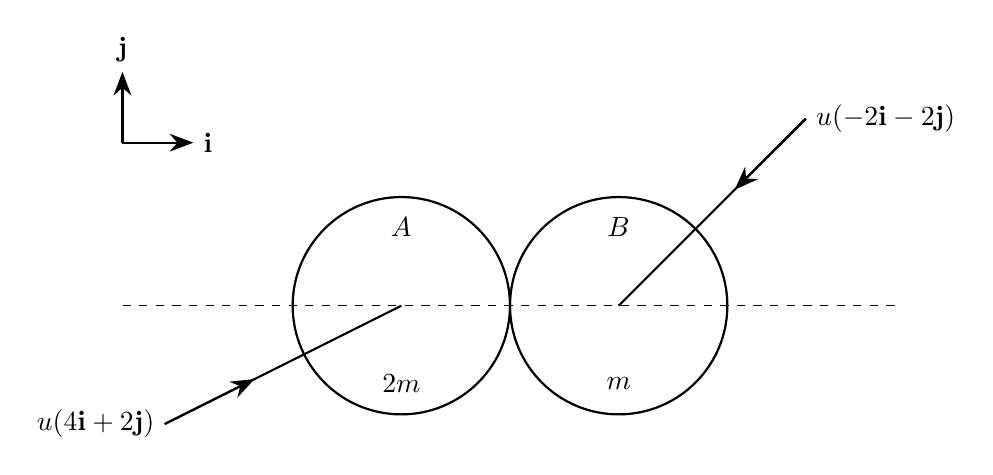
\begin{tikzpicture}[scale=1.2]
\def\rad{1.15}
\def\raylen{2.8}
\def\lineext{1.8}
\def\arrowfrac{0.38}
\def\basislen{0.75}
\pgfmathsetmacro{\adir}{atan2(2,4)}
\pgfmathsetmacro{\bdir}{atan2(-2,-2)}
\coordinate (A) at (0,0);
\coordinate (B) at ($(A)+(2*\rad,0)$);
\coordinate (L) at ($(A)+(-\rad-\lineext,0)$);
\coordinate (R) at ($(B)+(\rad+\lineext,0)$);
\coordinate (Ain) at ($(A)+({\adir+180}:\raylen)$);
\coordinate (Bin) at ($(B)+({\bdir+180}:\raylen)$);
\coordinate (Basis) at ($(L)+(0,1.5*\rad)$);
\draw[dashed,black] (L)--(R);
\foreach \p in {A,B} {\draw[thick,black] (\p) circle (\rad);}
\draw[thick,black] (Ain)--(A);
\draw[thick,black] (Bin)--(B);
\draw[-{Stealth[length=3mm]},thick,black] (Ain)--($(Ain)!\arrowfrac!(A)$) node[pos=0,left] {$u(4\mathbf{i}+2\mathbf{j})$};
\draw[-{Stealth[length=3mm]},thick,black] (Bin)--($(Bin)!\arrowfrac!(B)$) node[pos=0,right] {$u(-2\mathbf{i}-2\mathbf{j})$};
\draw[-{Stealth[length=3mm]},thick,black] (Basis)--++(\basislen,0) node[right] {$\mathbf{i}$};
\draw[-{Stealth[length=3mm]},thick,black] (Basis)--++(0,\basislen) node[above] {$\mathbf{j}$};
\node at ($(A)+(0,0.72*\rad)$) {$A$};
\node at ($(B)+(0,0.72*\rad)$) {$B$};
\node at ($(A)+(0,-0.72*\rad)$) {$2m$};
\node at ($(B)+(0,-0.72*\rad)$) {$m$};
\end{tikzpicture}
\end{figure}


Two smooth uniform spheres $A$ and $B$ of equal radius have masses $2m$ and $m$ respectively. They collide obliquely on a smooth horizontal surface. The unit vector $\mathbf{i}$ is directed along the line of centres from $A$ towards $B$ at impact, and $\mathbf{j}$ is perpendicular to $\mathbf{i}$ in the horizontal surface. \\

Immediately before the collision, the velocities of $A$ and $B$ are $u(4\mathbf{i}+2\mathbf{j})$ and $u(-2\mathbf{i}-2\mathbf{j})$ respectively, where $u>0$. The coefficient of restitution between the spheres is $e$, where $0\leq e\leq1$. \\
\begin{enumerate}[label=\textbf{(\alph*)}]
\item Find the velocity of each sphere immediately after the collision in terms of $u$ and $e$. \marks{5} \\
\item The velocities of the spheres immediately after the collision are perpendicular. Find the two possible values of $e$ and, for each value, calculate the total kinetic energy lost in the collision in terms of $m$ and $u$. \marks{6} \\
\end{enumerate}

\newpage

% ---- Question 5 ----
\questionitem
% [Source: _QBT__Oblique_Collisions_of_Smooth_Spheres, Q5]

\begin{figure}[H]
    \centering
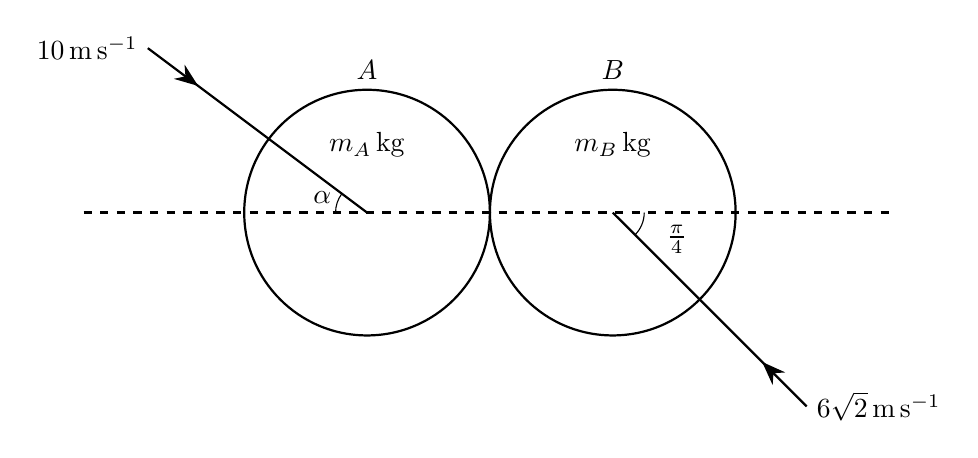
\begin{tikzpicture}[scale=1.2]
\def\rad{1.3}
\def\raylen{2.9}
\def\extend{1.7}
\def\massheight{0.55}
\pgfmathsetmacro{\alphaang}{atan(3/4)}
\coordinate (A) at (0,0);
\coordinate (B) at ($(A)+(2*\rad,0)$);
\coordinate (AL) at ($(A)+(180:\rad)$);
\coordinate (BR) at ($(B)+(0:\rad)$);
\coordinate (AS) at ($(A)+({180-\alphaang}:\raylen)$);
\coordinate (BS) at ($(B)+(-45:\raylen)$);
\draw[thick,black,dashed] ($(AL)+(-\extend,0)$) -- ($(BR)+(\extend,0)$);
\foreach \P in {A,B} {
  \draw[thick,black] (\P) circle (\rad);
  \node[above] at ($(\P)+(0,\rad)$) {$\P$};
}
\node at ($(A)+(0,\massheight*\rad)$) {$m_A\,\mathrm{kg}$};
\node at ($(B)+(0,\massheight*\rad)$) {$m_B\,\mathrm{kg}$};
\tikzset{incoming/.style={thick,black,postaction={decorate},decoration={markings,mark=at position 0.23 with {\arrow{Stealth[length=3mm]}}}}}
\draw[incoming] (AS) -- (A) node[pos=0,left] {$10\,\mathrm{m\,s^{-1}}$};
\draw[incoming] (BS) -- (B) node[pos=0,right] {$6\sqrt{2}\,\mathrm{m\,s^{-1}}$};
\pic["$\alpha$",draw,angle radius=4mm,angle eccentricity=1.5] {angle=AS--A--AL};
\pic["$\frac{\pi}{4}$",draw,angle radius=4mm,angle eccentricity=2.2] {angle=BS--B--BR};
\end{tikzpicture}
\end{figure}


Two smooth uniform spheres $A$ and $B$, of equal radius and masses $m_A\,\mathrm{kg}$ and $m_B\,\mathrm{kg}$ respectively, collide on a smooth horizontal surface. The diagram above shows their velocities immediately before impact, viewed from above. \\

Immediately before the collision, $A$ has speed $10\,\mathrm{m\,s^{-1}}$ and moves downwards and to the right at an acute angle $\alpha$ to the line of centres, where $\tan\alpha=\dfrac{3}{4}$. Sphere $B$ has speed $6\sqrt{2}\,\mathrm{m\,s^{-1}}$ and moves upwards and to the left at an angle $\dfrac{\pi}{4}$ to the line of centres. \\

Immediately after the collision, $B$ moves upwards and to the right at an acute angle $\beta$ to the rightward line of centres, where $\tan\beta=2$. The coefficient of restitution between the spheres is $e$, where $0\leq e\leq1$. \\
\begin{enumerate}[label=\textbf{(\alph*)}]
\item Find the complete interval of possible values of $\dfrac{m_B}{m_A}$. State which endpoint corresponds to a perfectly elastic collision. \marks{7} \\
\item Given that $m_A=3$ and $m_B=4$, find the total loss of kinetic energy in the collision. \marks{4} \\
\end{enumerate}

\newpage

% ---- Question 6 ----
\questionitem
% [Source: _QBT__Oblique_Collisions_of_Smooth_Spheres, Q6]

In this question, $\mathbf{i}$ and $\mathbf{j}$ are perpendicular unit vectors in a horizontal plane. \\

Two smooth uniform spheres $P$ and $Q$, of equal radius, have masses $0.4\,\mathrm{kg}$ and $0.5\,\mathrm{kg}$ respectively. They move on a smooth horizontal surface and collide obliquely. \\

Immediately before the collision, their velocities are
\[
\mathbf{u}_P=(0.8\mathbf{i}+4.4\mathbf{j})\,\mathrm{m\,s^{-1}},\qquad \mathbf{u}_Q=(1.2\mathbf{i}-3.4\mathbf{j})\,\mathrm{m\,s^{-1}}
\] \\
At the instant of collision, the vector from the centre of $P$ to the centre of $Q$ is parallel to $3\mathbf{i}+4\mathbf{j}$. \\

The coefficient of restitution between the spheres is $e$. The collision deflects the direction of motion of $P$ through $90^\circ$. \\
\begin{enumerate}[label=\textbf{(\alph*)}]
\item Find $e$. \marks{8} \\
\item Find the velocity of $Q$ immediately after the collision. Hence find the angle through which its direction of motion is deflected, giving your answer to the nearest $0.1^\circ$. \marks{6} \\
\item State how you have used the fact that the spheres have equal radii. \marks{1} \\
\end{enumerate}

\newpage

% ---- Question 7 ----
\questionitem
% [Source: _QBT__Oblique_Collisions_of_Smooth_Spheres, Q7]

Two smooth uniform spheres $P$ and $Q$ have equal radii and masses $0.4\,\mathrm{kg}$ and $0.6\,\mathrm{kg}$ respectively. They move on a smooth horizontal surface and collide obliquely. \\

Immediately before the collision, their velocities are
\[
\mathbf{u}_P=(6\mathbf{i}+2\mathbf{j})\,\mathrm{m\,s^{-1}},\qquad \mathbf{u}_Q=(-2\mathbf{i}+2\mathbf{j})\,\mathrm{m\,s^{-1}}
\] \\
where $\mathbf{i}$ and $\mathbf{j}$ are perpendicular horizontal unit vectors. \\

At the instant of impact, the vector from the centre of $P$ to the centre of $Q$ is a positive multiple of $\mathbf{i}+\mathbf{j}$. The total kinetic energy of the two spheres decreases by $2.88\,\mathrm{J}$ during the collision. \\
\begin{enumerate}[label=\textbf{(\alph*)}]
\item Find
\begin{enumerate}[label=(\roman*)]
\item the velocity of $P$ immediately after the collision,
\item the velocity of $Q$ immediately after the collision,
\item the coefficient of restitution between the spheres.
\end{enumerate}
Justify your answers, explaining which velocity components are unchanged by the collision. \marks{12} \\
\item Find the angle through which the direction of motion of $P$ is deflected by the collision. Give your answer in degrees to one decimal place. \marks{3} \\
\end{enumerate}

\newpage

% ---- Question 8 ----
\questionitem
% [Source: _QBT__Oblique_Collisions_of_Smooth_Spheres, Q8]

\begin{figure}[H]
    \centering
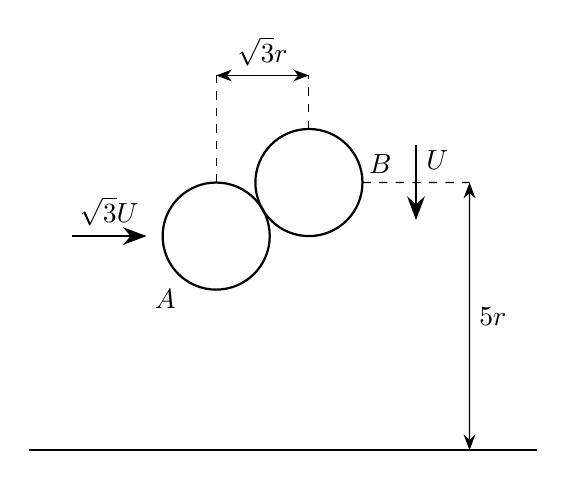
\begin{tikzpicture}[scale=0.85]
\def\rad{0.8}
\def\heightA{4}
\def\heightB{5}
\def\dimLevel{7}
\def\heightOffset{3}
\def\groundLeft{-3.5}
\def\groundRight{6}
\def\arrowOffset{2}
\def\arrowHalfLength{0.7}
\pgfmathsetmacro{\sep}{sqrt(3)*\rad}
\coordinate (A) at (0,\heightA*\rad);
\coordinate (B) at (\sep,\heightB*\rad);
\coordinate (Adim) at (0,\dimLevel*\rad);
\coordinate (Bdim) at (\sep,\dimLevel*\rad);
\coordinate (Htop) at ($(B)+(\heightOffset*\rad,0)$);
\coordinate (Hbase) at (Htop |- 0,0);
\coordinate (VA) at ($(A)+(-\arrowOffset*\rad,0)$);
\coordinate (VB) at ($(B)+(\arrowOffset*\rad,0)$);
\draw[thick, black] (\groundLeft*\rad,0) -- (\groundRight*\rad,0);
\draw[thick, black] (A) circle (\rad);
\draw[thick, black] (B) circle (\rad);
\draw[-{Stealth[length=3mm]}, thick, black] ($(VA)+(-\arrowHalfLength*\rad,0)$) -- ($(VA)+(\arrowHalfLength*\rad,0)$) node[midway, above] {$\sqrt{3}U$};
\draw[-{Stealth[length=3mm]}, thick, black] ($(VB)+(0,\arrowHalfLength*\rad)$) -- ($(VB)+(0,-\arrowHalfLength*\rad)$) node[pos=0.2, right] {$U$};
\draw[dashed] ($(A)+(0,\rad)$) -- (Adim);
\draw[dashed] ($(B)+(0,\rad)$) -- (Bdim);
\draw[{Stealth[length=2mm]}-{Stealth[length=2mm]}] (Adim) -- (Bdim) node[midway, above] {$\sqrt{3}r$};
\draw[dashed] ($(B)+(\rad,0)$) -- (Htop);
\draw[{Stealth[length=2mm]}-{Stealth[length=2mm]}] (Hbase) -- (Htop) node[midway, right] {$5r$};
\node[below left] at ($(A)+(235:\rad)$) {$A$};
\node[right] at ($(B)+(20:\rad)$) {$B$};
\end{tikzpicture}
\end{figure}


Two uniform smooth spheres, $A$ and $B$, have equal radius $r$ and masses $2m$ and $3m$ respectively. They collide while moving freely above a horizontal plane. The diagram above shows the spheres at the instant of impact, with their centres and velocities in the same vertical plane. \\

At impact, the centres of $A$ and $B$ are at heights $4r$ and $5r$ respectively above the horizontal plane, and their horizontal separation is $\sqrt{3}r$. Immediately before impact, $A$ has velocity $\sqrt{3}U$ horizontally to the right and $B$ has velocity $U$ vertically downwards, where $U>0$. \\
\begin{enumerate}[label=\textbf{(\alph*)}]
\item Show that the line of centres makes an angle of $30^\circ$ with the horizontal, and that the speed of approach along this line is $2U$. \marks{2} \\
\end{enumerate}
The coefficient of restitution between the spheres is $\dfrac{2}{3}$. After the collision, $B$ moves freely under gravity and does not collide with $A$ again. Air resistance is negligible and the acceleration due to gravity is $g$. \\
\begin{enumerate}[label=\textbf{(\alph*)}, resume]
\item Find, in terms of $U$, $r$ and $g$, the exact time from the collision until $B$ first touches the horizontal plane. \marks{7} \\
\end{enumerate}

\newpage

% ---- Question 9 ----
\questionitem
% [Source: _QBT__Oblique_Collisions_of_Smooth_Spheres, Q9]

In this question, $\mathbf{i}$ and $\mathbf{j}$ are unit vectors due east and due north respectively. \\

Two smooth uniform spheres $P$ and $Q$, each of radius $2.5\,\mathrm{m}$, move on a smooth horizontal surface. Their masses are $3\,\mathrm{kg}$ and $2\,\mathrm{kg}$ respectively. At time $t=0$, the centre of $Q$ is $7\,\mathrm{m}$ east and $26\,\mathrm{m}$ north of the centre of $P$. Their velocities are
\[
\mathbf{u}_P=(2\mathbf{i}+6\mathbf{j})\,\mathrm{m\,s^{-1}},\qquad \mathbf{u}_Q=-5\mathbf{j}\,\mathrm{m\,s^{-1}}
\] \\
\begin{enumerate}[label=\textbf{(\alph*)}]
\item Show that the spheres will collide and determine the time at which they first make contact. \marks{5} \\
\end{enumerate}
Immediately after the collision, the speed of $Q$ is $3\sqrt{5}\,\mathrm{m\,s^{-1}}$. \\
\begin{enumerate}[label=\textbf{(\alph*)}, resume]
\item Determine the coefficient of restitution between the spheres and hence find the velocity of $P$ immediately after the collision. \marks{9} \\
\item Find, in vector form, the impulse required to bring $P$ to rest after the collision. Calculate the angle this impulse makes with the eastward direction, stating whether it acts north or south of east. \marks{4} \\
\end{enumerate}

\newpage

% ---- Question 10 ----
\questionitem
% [Source: _QBT__Oblique_Collisions_of_Smooth_Spheres, Q10]

Two small uniform smooth spheres $A$ and $B$ have equal radii and masses $m$ and $\lambda m$ respectively, where $\lambda>0$. They move on a smooth horizontal surface. The unit vectors $\mathbf{i}$ and $\mathbf{j}$ are perpendicular and lie in the surface. \\

Immediately before an oblique collision, the velocities of $A$ and $B$ are $u(4\mathbf{i}+\mathbf{j})$ and $u(-\mathbf{i}+2\mathbf{j})$ respectively, where $u>0$. At impact, the line of centres is parallel to $\mathbf{i}+\mathbf{j}$, with $B$ lying in the direction $\mathbf{i}+\mathbf{j}$ from $A$. \\

The coefficient of restitution between the spheres is $e$, where $0\leq e\leq1$. \\
\begin{enumerate}[label=\textbf{(\alph*)}]
\item
\begin{enumerate}[label=(\roman*)]
\item Explain why the impulse exerted by $A$ on $B$ is parallel to $\mathbf{i}+\mathbf{j}$. \marks{1} \\
\item Determine the velocity of each sphere immediately after the collision in terms of $u$, $\lambda$ and $e$, giving your answers in terms of $\mathbf{i}$ and $\mathbf{j}$. \marks{7} \\
\end{enumerate}
\end{enumerate}
The loss of kinetic energy in the collision is $mu^2$. Immediately after the collision, the component of the velocity of $A$ in the direction $\mathbf{i}+\mathbf{j}$ is negative. \\
\begin{enumerate}[label=\textbf{(\alph*)}, resume]
\item Determine the range of possible values of $\lambda$ consistent with both of these conditions. \marks{7} \\
\end{enumerate}

\end{enumerate}
\end{document}
